\section{Simulations}
\label{sec:simulations}

We evaluate our approach on the running example, and on a 4D flexible joint manipulator.
We implemented the RMPC controller of Algorithm ?? in MATLAB
The set computations were done using the MPT Toolbox \cite{MPT3}, and the invariant set computations using the Matlab Invariant Set Toolbox \cite{IST}. 
The reachability computations for $\oaXset{k+j}{k}$ were performed on the linear dynamics and mapped back to $x$-space as described in Sec. \ref{sec:transforming x to z}.
The RMPC optimizations were performed by Gurobi \cite{gurobi}.

\subsection{Running example}

For the running example of Eq. ??, we discretize the feedback linearized system at 10Hz and formulate the controller with a horizon of $N=15$ steps. 
The cost function has parameters $Q=I$ and $R=10^-2$.
The state trajectories for the feedback linearized system are shown in Fig. ??, and those of the nonlinear system in Fig ??.
Note that the latter converges to the equilibrium 0. 
%The input for the feedback linearized system is shown in Fig. ?? along with its upper and lower rectangular bounds computed online, denoted as $\oa{V}_{k|k}$ and $\ua{V}_{k|k}$ respectively, which make up the input constraint set at time $k$.
%Also shown is the global inner approximation $V_{inner-global}$ for the input $v$. 
%It is worth noting that the bounds computed online allow for much more control action than the conservative $V_{inner-global}$. 
The input $u$ is shown in Fig. ??, and it can be noted that $u_k \in U$ for all $k$.

\begin{figure}
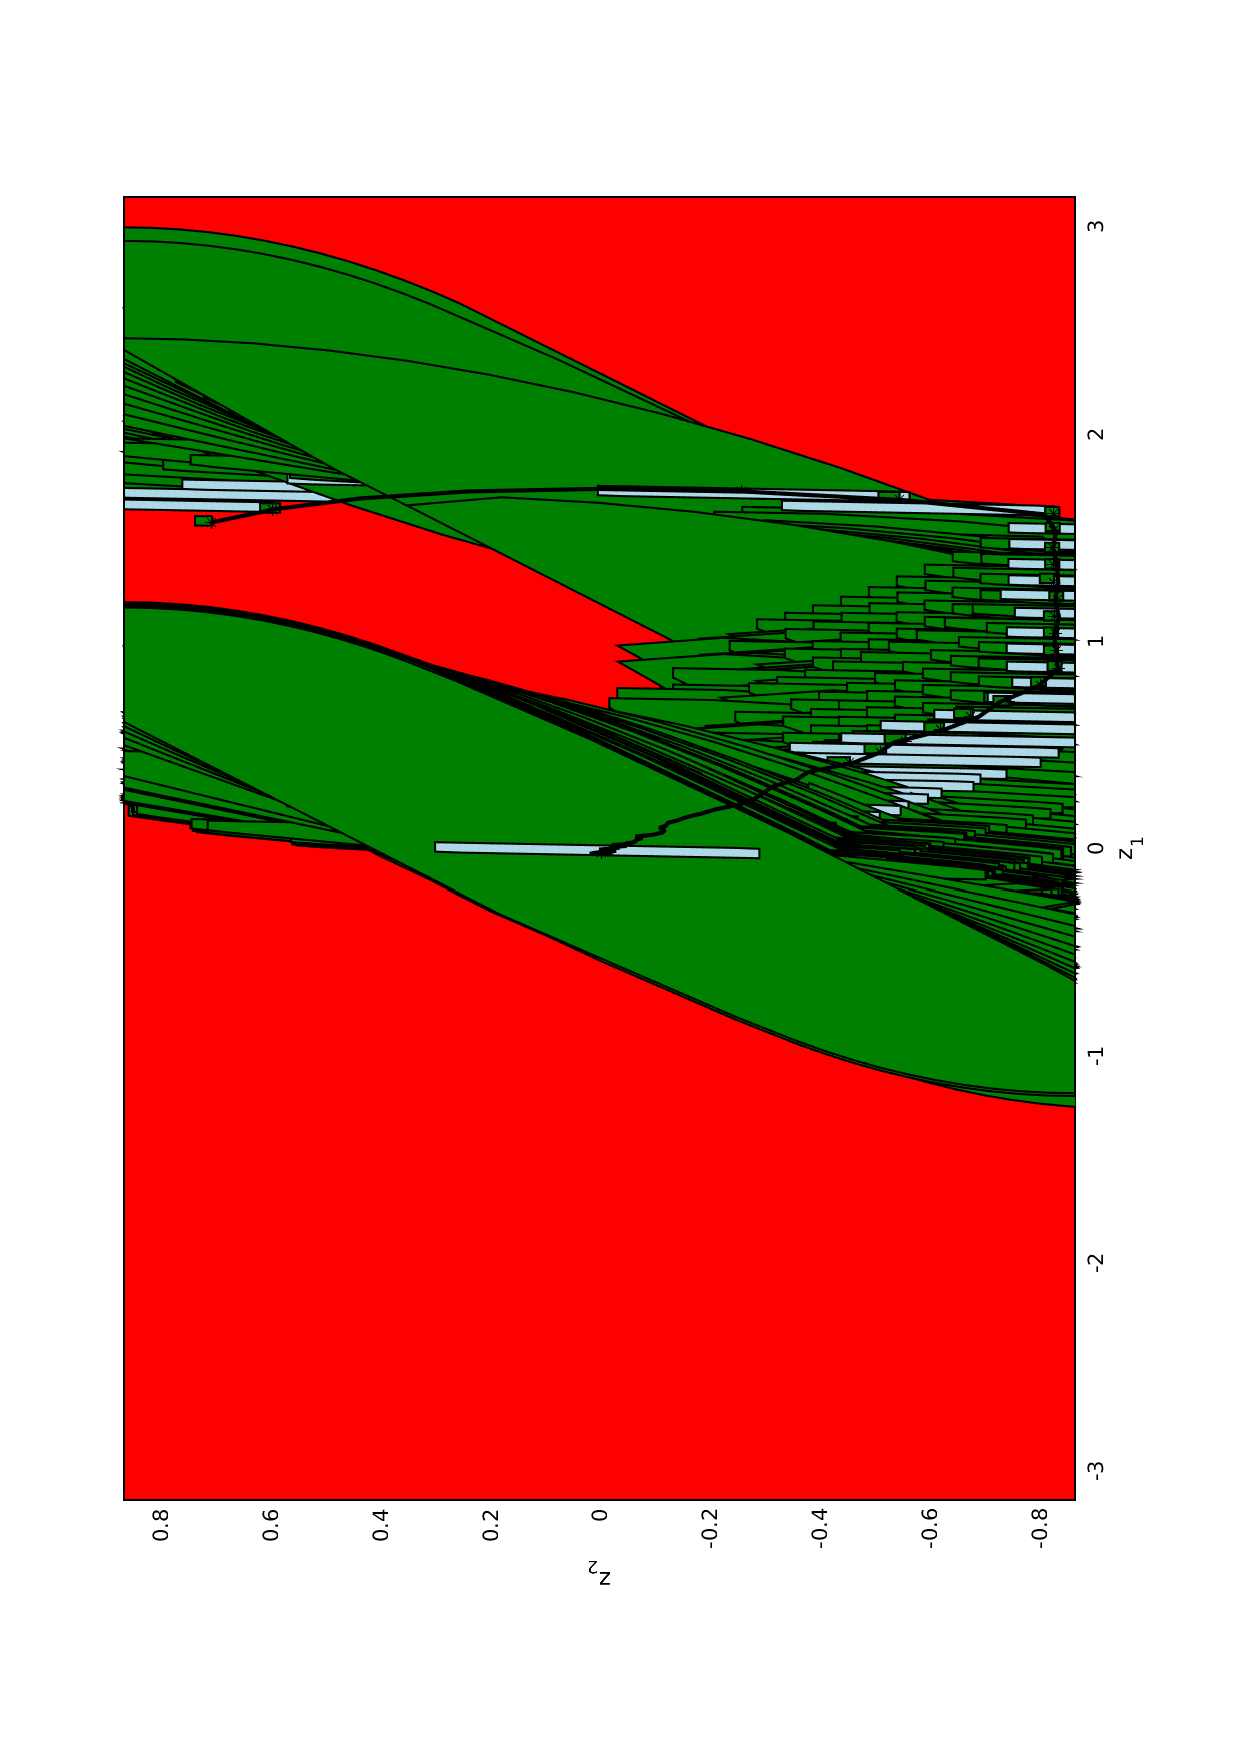
\includegraphics[angle=270,width=0.49\textwidth]{figs/z_trajectory_new.pdf}
\caption{Evolution of $z_1$ and $z_2$, shown by the solid black line, inside the set Z (in red). The green sets are the reach sets $\oa{Z}_{k+i|k},\forall i=1,\dotsc,N, \forall k$. The light blue set is the one step ahead reach set $\oa{Z}_{k+1|k},\forall k$.}
\label{fig:z_new_toy}
\end{figure}




\subsection{Single link flexible joint manipulator}

As a more complex example, we consider the single link flexible manipulator dynamics, which have also been covered in ??,??,??. The non-linear plant dynamics are given as:

\begin{equation}
\begin{bmatrix} \dot{x}_1 \\ \dot{x}_2 \\ \dot{x}_3 \\ \dot{x}_4    \end{bmatrix} = \begin{bmatrix} x_2 \\ -\frac{mgl}{I}sin(x_1) - \frac{k}{I}(x_1-x_3)  \\ x_4 \\ \frac{k}{J}(x_1-x_3)  \end{bmatrix} + \begin{bmatrix} 0 \\ 0 \\ 0 \\ \frac{1}{J} \end{bmatrix}u
\end{equation}

This models a system where a motor, with an angular moment of inertia $J$,  is coupled to a uniform thin bar of of mass $m$, length $l$ and moment of inertia $I$, through a flexible link, where the flexibility is modeled by a torsional string with stiffness $k$. Here, $x_2$ is the angle of the motor shaft and $x_4$ the rate. The angle of the bar at the end of the flexible link is $x_1$ and its rate  is $x_3$. The input to the system is the motor torque, given by $u$. 

Without getting into the details of the feedback linearization, the diffeomorphism mapping the states of the non-linear system to the feedback linearized system, which is valid in the domain $x \in \mathbb{R}^4$ is given by:

\begin{equation}
z = T(x) = \begin{bmatrix} x_1 \\ x_2 \\ -\frac{mgl}{I}sin(x_1) -\frac{k}{I}(x_1-x_3) \\ \frac{mgl}{I}x_2cos(x_1) - \frac{k}{I}(x_2-x_4)   \end{bmatrix}
\end{equation}

For the linearization of Eq. ??, where $\hat{z}_k = z_k + M(x_k)e_k$, the matrix $M(x_k)$ is given by:
\begin{equation}
M(x_k) = \begin{bmatrix} 1&0&0&0 \\ 0&1&0&0 \\ -\frac{mgl}{I} cos(x_{1k}) -\frac{k}{I} &0 &\frac{k}{I} &0 \\ \frac{mgl}{I}x_{2k}sin(x_{1k}) & -\frac{mgl}{I} cos(x_{1k}) - \frac{k}{I} & 0 & \frac{k}{I}     \end{bmatrix}
\end{equation}

Also, the input to the feedback linearized system is given by:

\begin{subequations}
\label{eq:fblin_inp}
\begin{align}
v&=\beta u+ \alpha(x) \\
&\text{Where,} \nonumber \\
\beta&=\frac{k}{IJ} \\
\alpha(x)&=\frac{mgl}{I}x_2^2sin(x_1) + \frac{k^2}{IJ}(x_1-x_3) \nonumber \\
&- (\frac{mgl}{I}cos(x_1)-\frac{k}{I})(\frac{mgl}{I}sin(x_1)+\frac{k}{I}(x_1-x_3))
\end{align}
\end{subequations}

Under this feedback linearizing input and the diffeomorphism $T$, the feedback linearized systems has the dynamics:

\begin{subequations}
\begin{align}
\label{eq:fblin_manip}
\dot{z_1} &= z_2 \\
\dot{z_2} &= z_3 \\
\dot{z_3} &= z_4 \\
\dot{z_4} &= v
\end{align}
\end{subequations}

The safe set for the states $X$, is defined as follows, 
\begin{equation}
 -\begin{bmatrix} \pi/4  \\ \pi/4  \\ \pi \\ \pi \end{bmatrix} \leq x \leq \begin{bmatrix} \pi/4  \\ \pi/4  \\ \pi \\ \pi \end{bmatrix}
\end{equation}

Where the angles and their derivatives are in radians and radians per second respectively. Note, the safe set places a smaller degree of freedom on the range and angular velocities of the rod compared to the motor shaft.
The limits on the input torque, in $Nm$, $u$, are given by the set $U = u :-10 \leq u \leq 10$. The estimation for the state estimation, where $\hat{x} = x + e$ are given by $E = e:-\pi /180 \leq e \leq \pi /180 $, where the units are radians and radians per second accordingly. 

From Eq. \ref{eq:fblin_inp}, we can compute $V_{inner-global} =v: max_{x\in X}\alpha(x) + \beta \underline{u} \leq v \leq min_{x\in X}\alpha(x) + \beta \overline{u}$. Since $X$ is a hyper rectangle, we can compute $\overline{\alpha}(x)_{X} \geq  max_{x\in X}\alpha(x)$ using interval arithmetic, and similarly $\underline{\alpha}(x)_{X} \leq  min_{x\in X}\alpha(x)$, and hence compute (an under-approximation of) $V_{inner-global}$. Here $\underline{u}=-10$ and $\overline{u}=10$ , the upper and lower limits on $u$ that define the set $U$.
Similarly for the input set underapproximation (Eq.??) computed online, we have $\underline{V}_{k+j|k} = v:   max_{x\in \oa{X}_{k+j|k}} \alpha(x) + \beta \underline{u} \leq v \leq  min_{x\in \oa{X}_{k+j|k}}\alpha(x) + \beta \overline{u}$. This set (an under-approximation of it) can also be computed online using interval arithmetic by over-approximating $\oa{x}_{k+j|k}$ by a hyper-rectangle. The constants, other than $g=9.8ms^{-2}$, for numerical simplicity are chosen as $m=1/9.8g$, $l=1m$, $J=1$ and $I=1$. For the cost function of Eq. ??, we choose $Q=I$ and $R=10^-2$. For our control algorithm, which is a discrete time algorithm, we discretize the feedback linearized system of Eq. \ref{eq:fblin_manip} at 10Hz, and formulate the controller for a horizon of $N=10$ steps.

The set of states for the feedback linearized system $Z$ (as computed by ??) is given by:

\begin{equation}
 -\begin{bmatrix} 0.5121  \\ 0.5121  \\ 2.5347 \\ 2.5603 \end{bmatrix} \leq z \leq \begin{bmatrix} 0.5121  \\ 0.5121  \\ 2.5347 \\ 2.5603 \end{bmatrix}
\end{equation}

Figures ??,?? shows the states of the feedback linearized system. As formulated, the states converge to the origin in the presence of estimation error, while respecting all constraints on them.

\begin{figure}
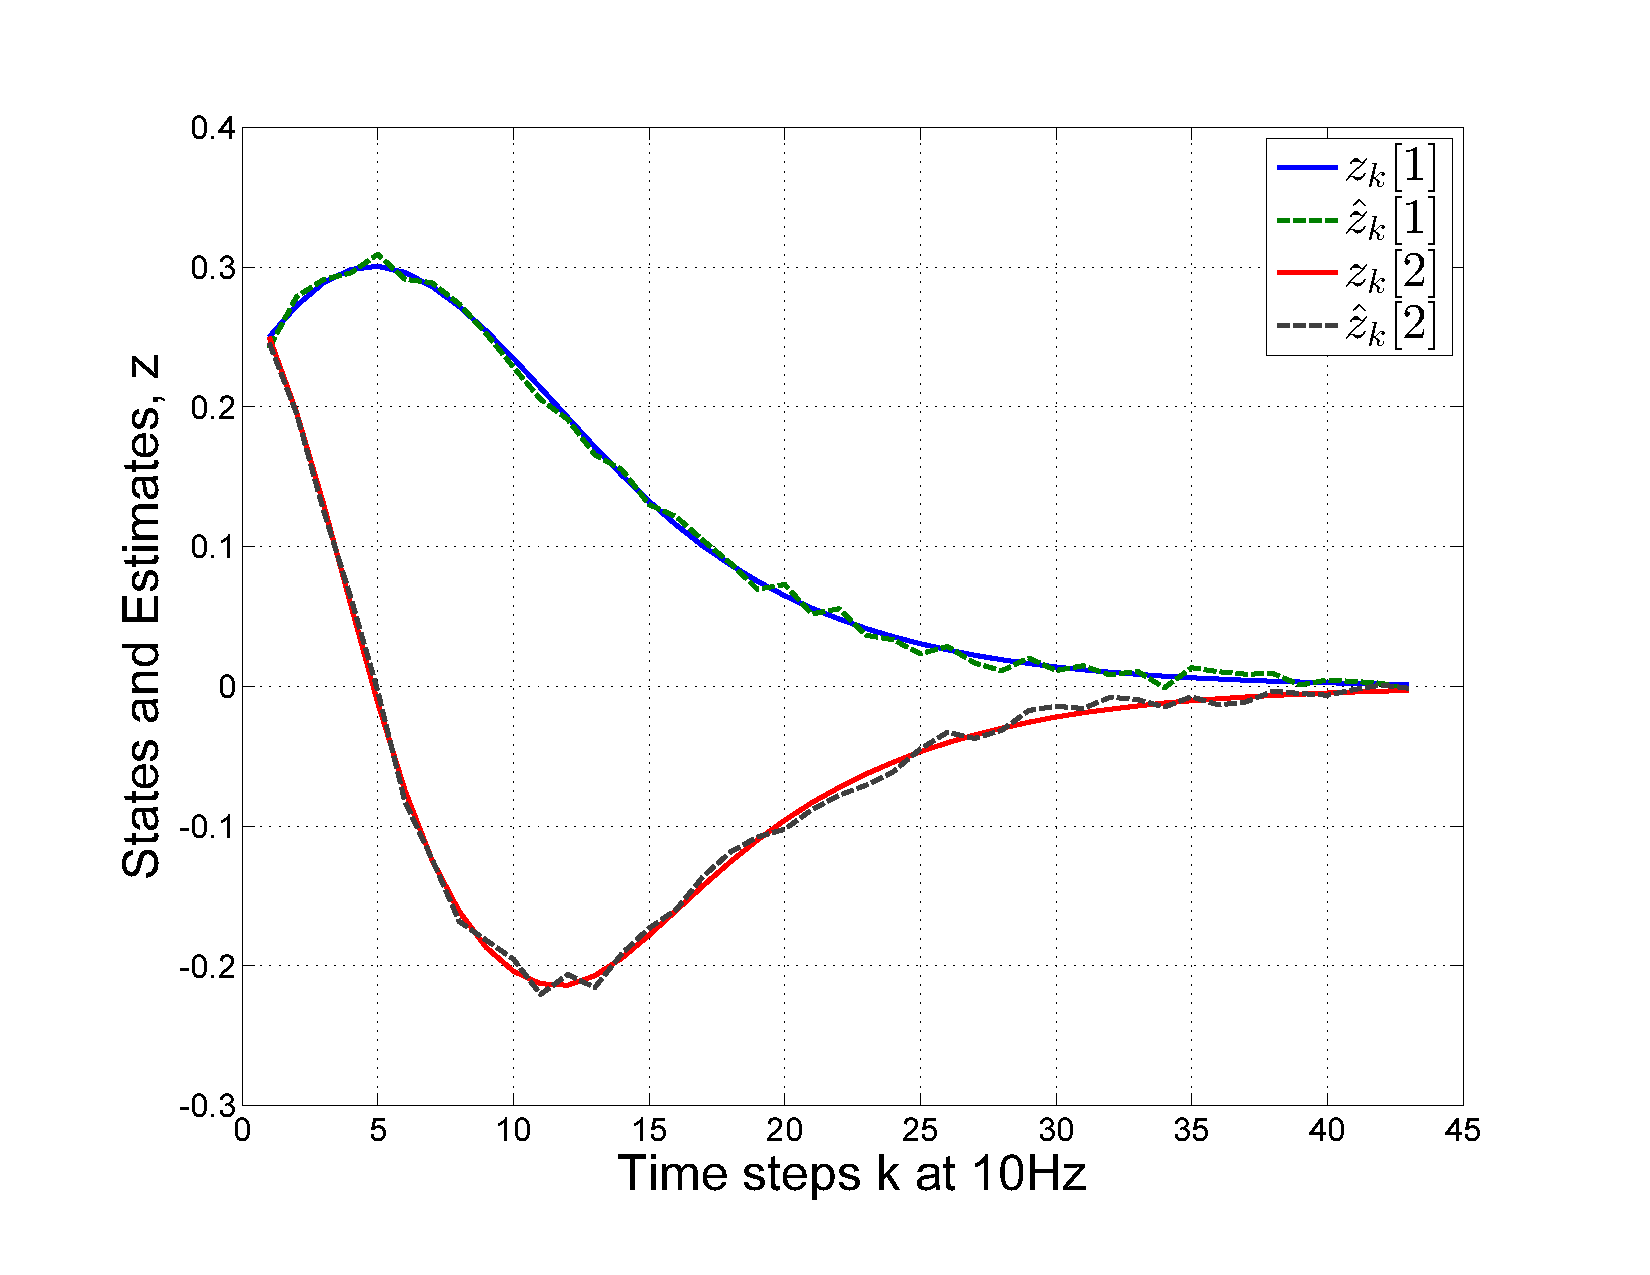
\includegraphics[width=0.49\textwidth]{figs/z_1n2_manip.pdf}
\caption{$z_1$ and $z_2$ and their estimates $\hat{z_1}, \, \hat{z_2}$ vs time. Note, these states are the same as $x_1$ and $x_2$ respectively, the angular position and velocities of the rod at the end of the manipulator.}
\label{fig:z_12}
\end{figure}

\begin{figure}
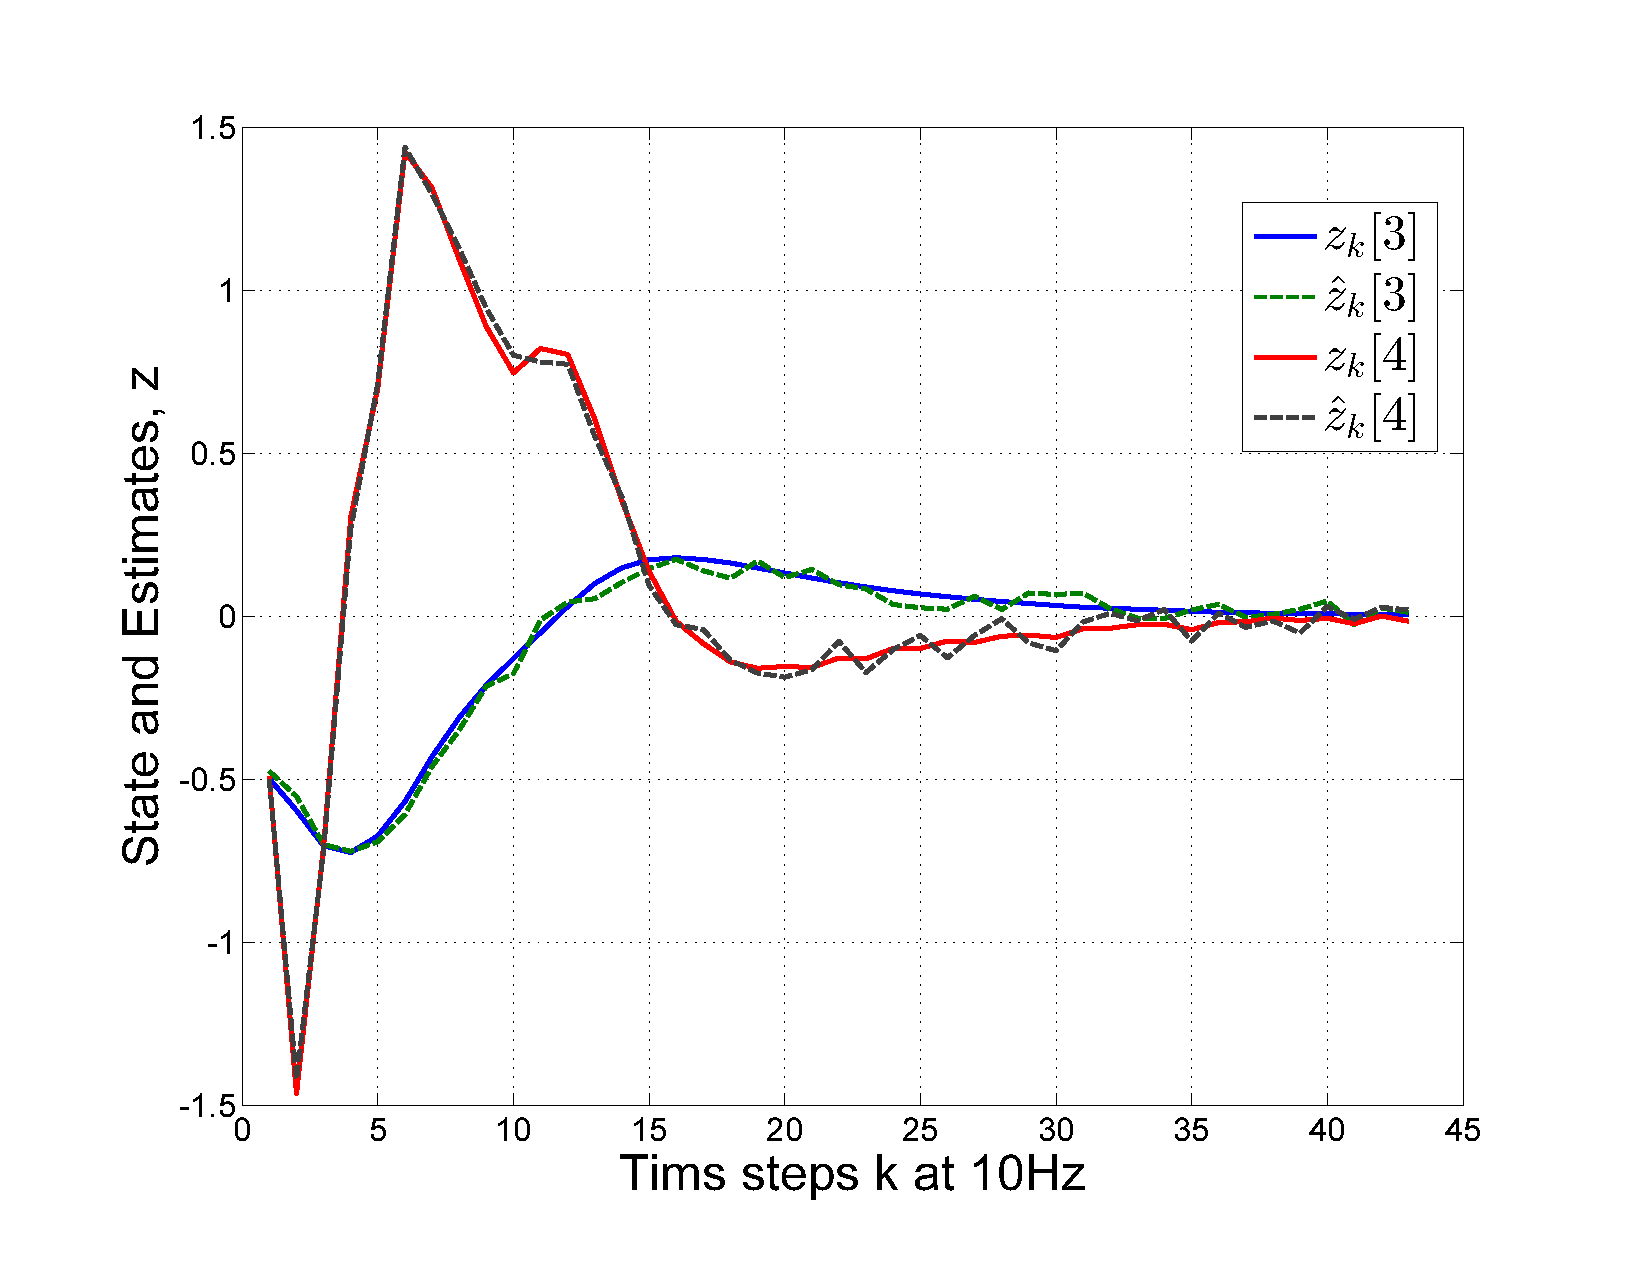
\includegraphics[width=0.49\textwidth]{figs/z_3n4_manip.pdf}
\caption{$z_3$ and $z_4$ and their estimates $\hat{z_3}, \, \hat{z_4}$ vs time. }
\label{fig:z_34}
\end{figure}

Figure ?? shows the 2 remaining states of the non-linear system, $x_3$ and $x_4$. They also converge to zero, showing that the non-linear has been stabilized while robustly respecting $x\in X$ under the presence of estimation error. Figure ?? shows the input to the feedback linearized system $v$ and its bounds, both the global inner approximation and the ones computed online. Note, similar to the toy proble, the bounds computed online allow for more control action compared to the conservative global inner approximation. Finally, Fig. ?? shows the actual input applied to the non-linear system (and its bounds), which robustly respects its constraints $u \in U$.

\begin{figure}
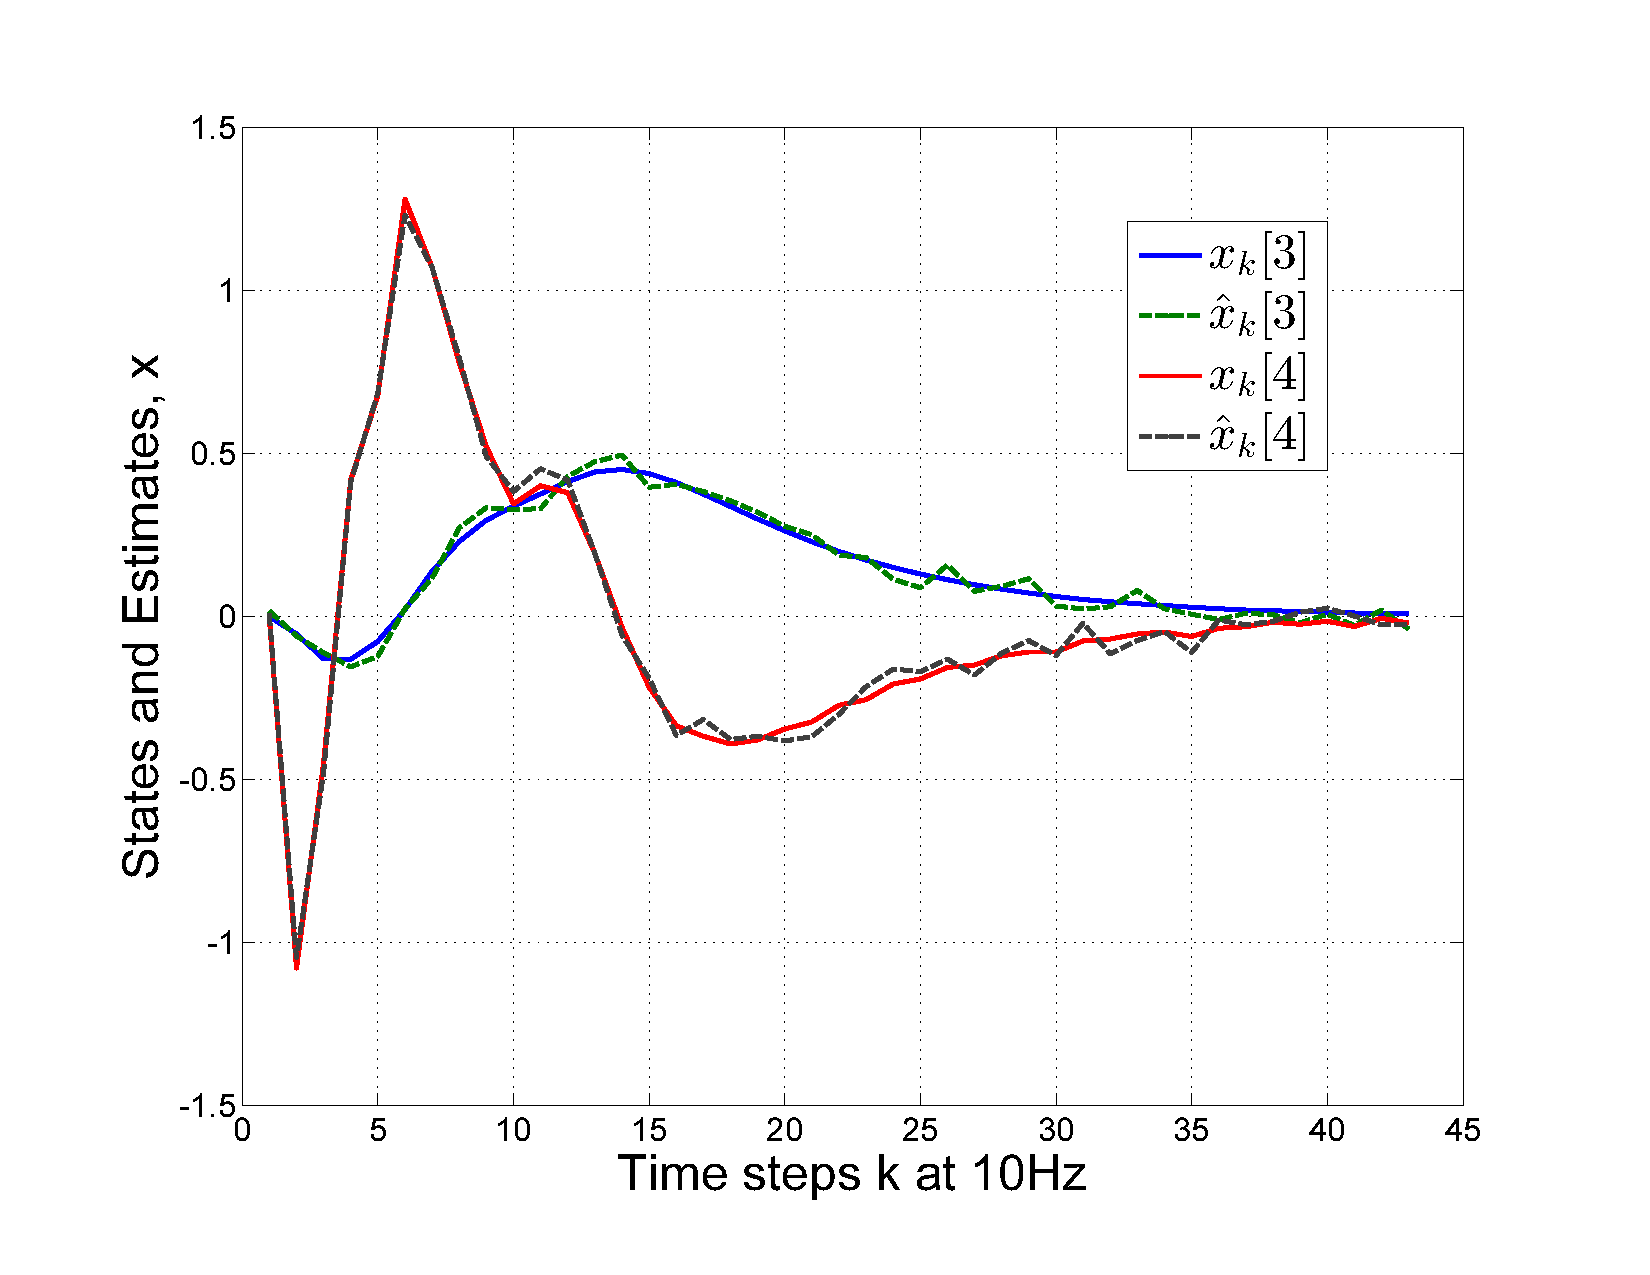
\includegraphics[width=0.49\textwidth]{figs/x_3n4_manip.pdf}
\caption{$x_3$ and $x_4$ and their estimates $\hat{x_3}, \, \hat{x_4}$ vs time. }
\label{fig:x_34}
\end{figure}

\begin{figure}
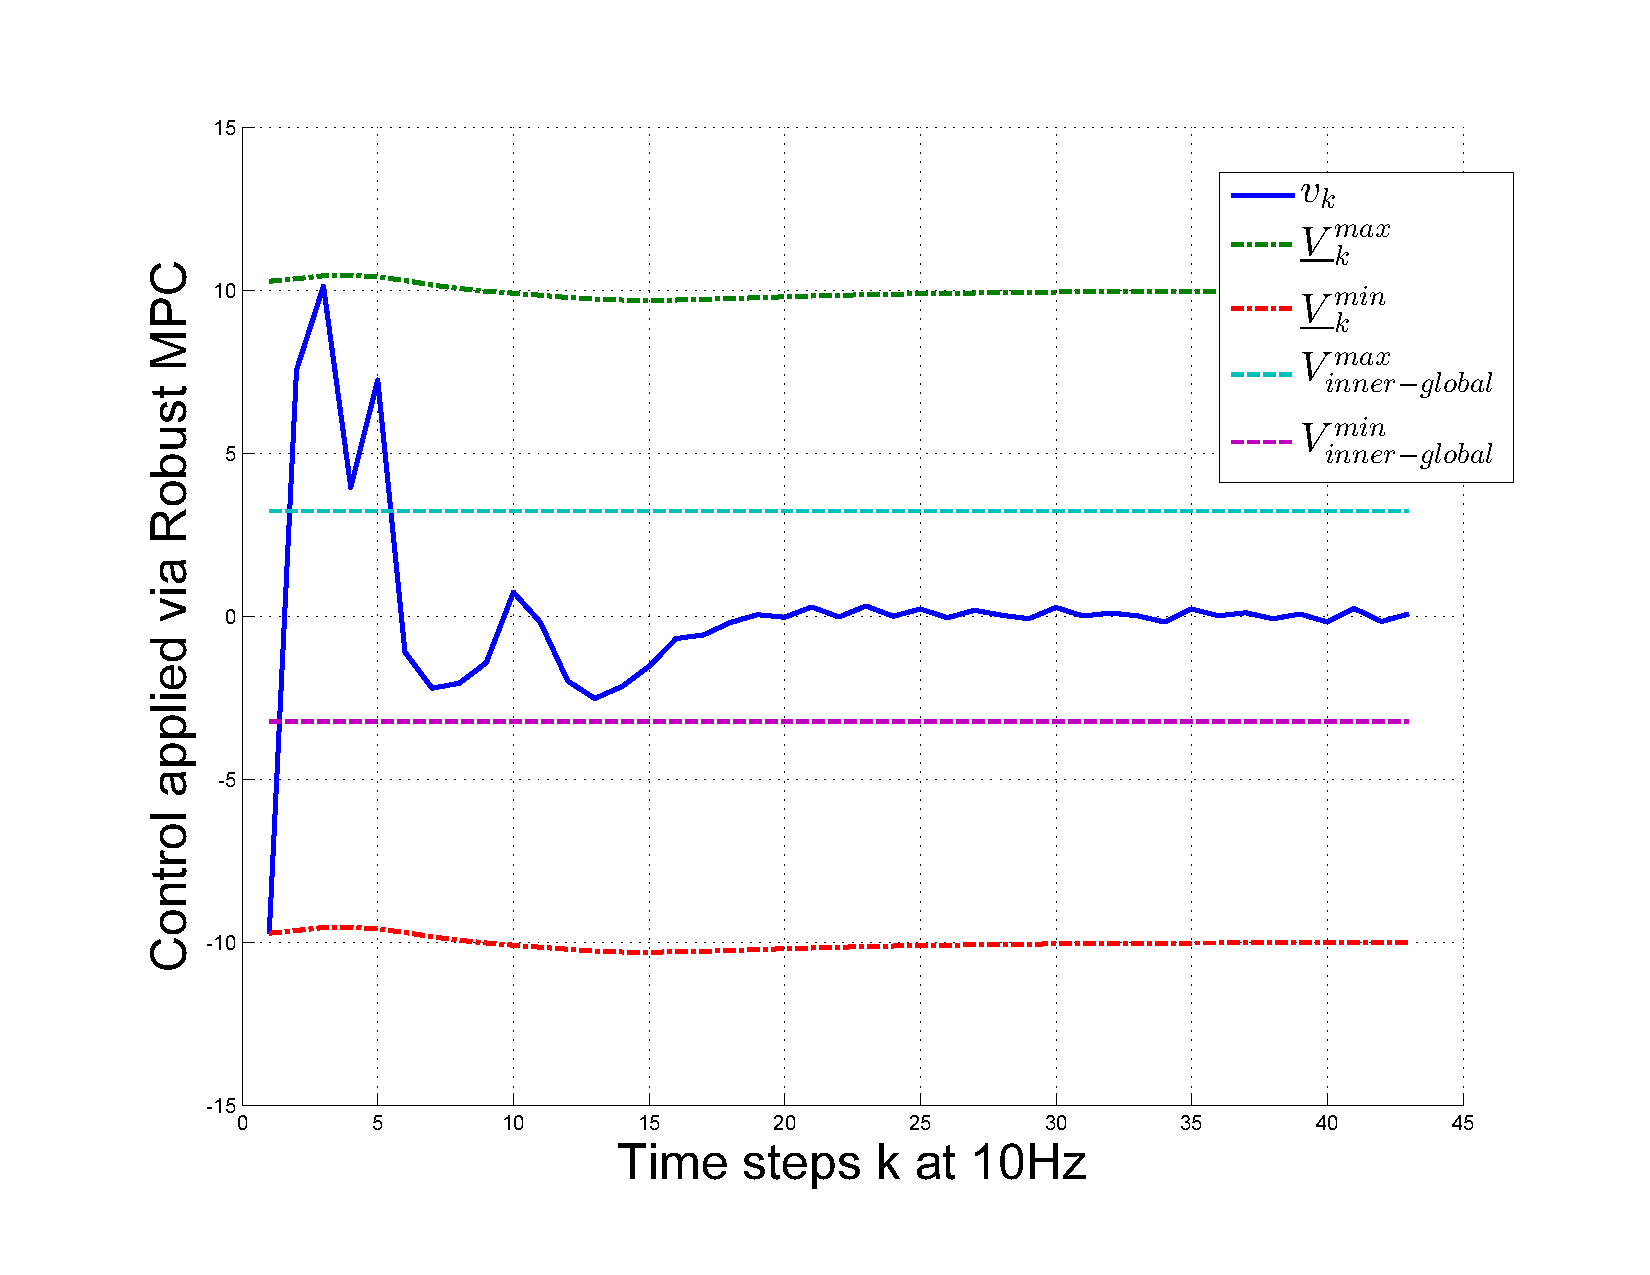
\includegraphics[width=0.49\textwidth]{figs/v_and_limits_manip.pdf}
\caption{Input to the feedback linearized system as computed by the control algorithm, and its bounds.}
\label{fig:v_and_limits}
\end{figure}

\begin{figure}
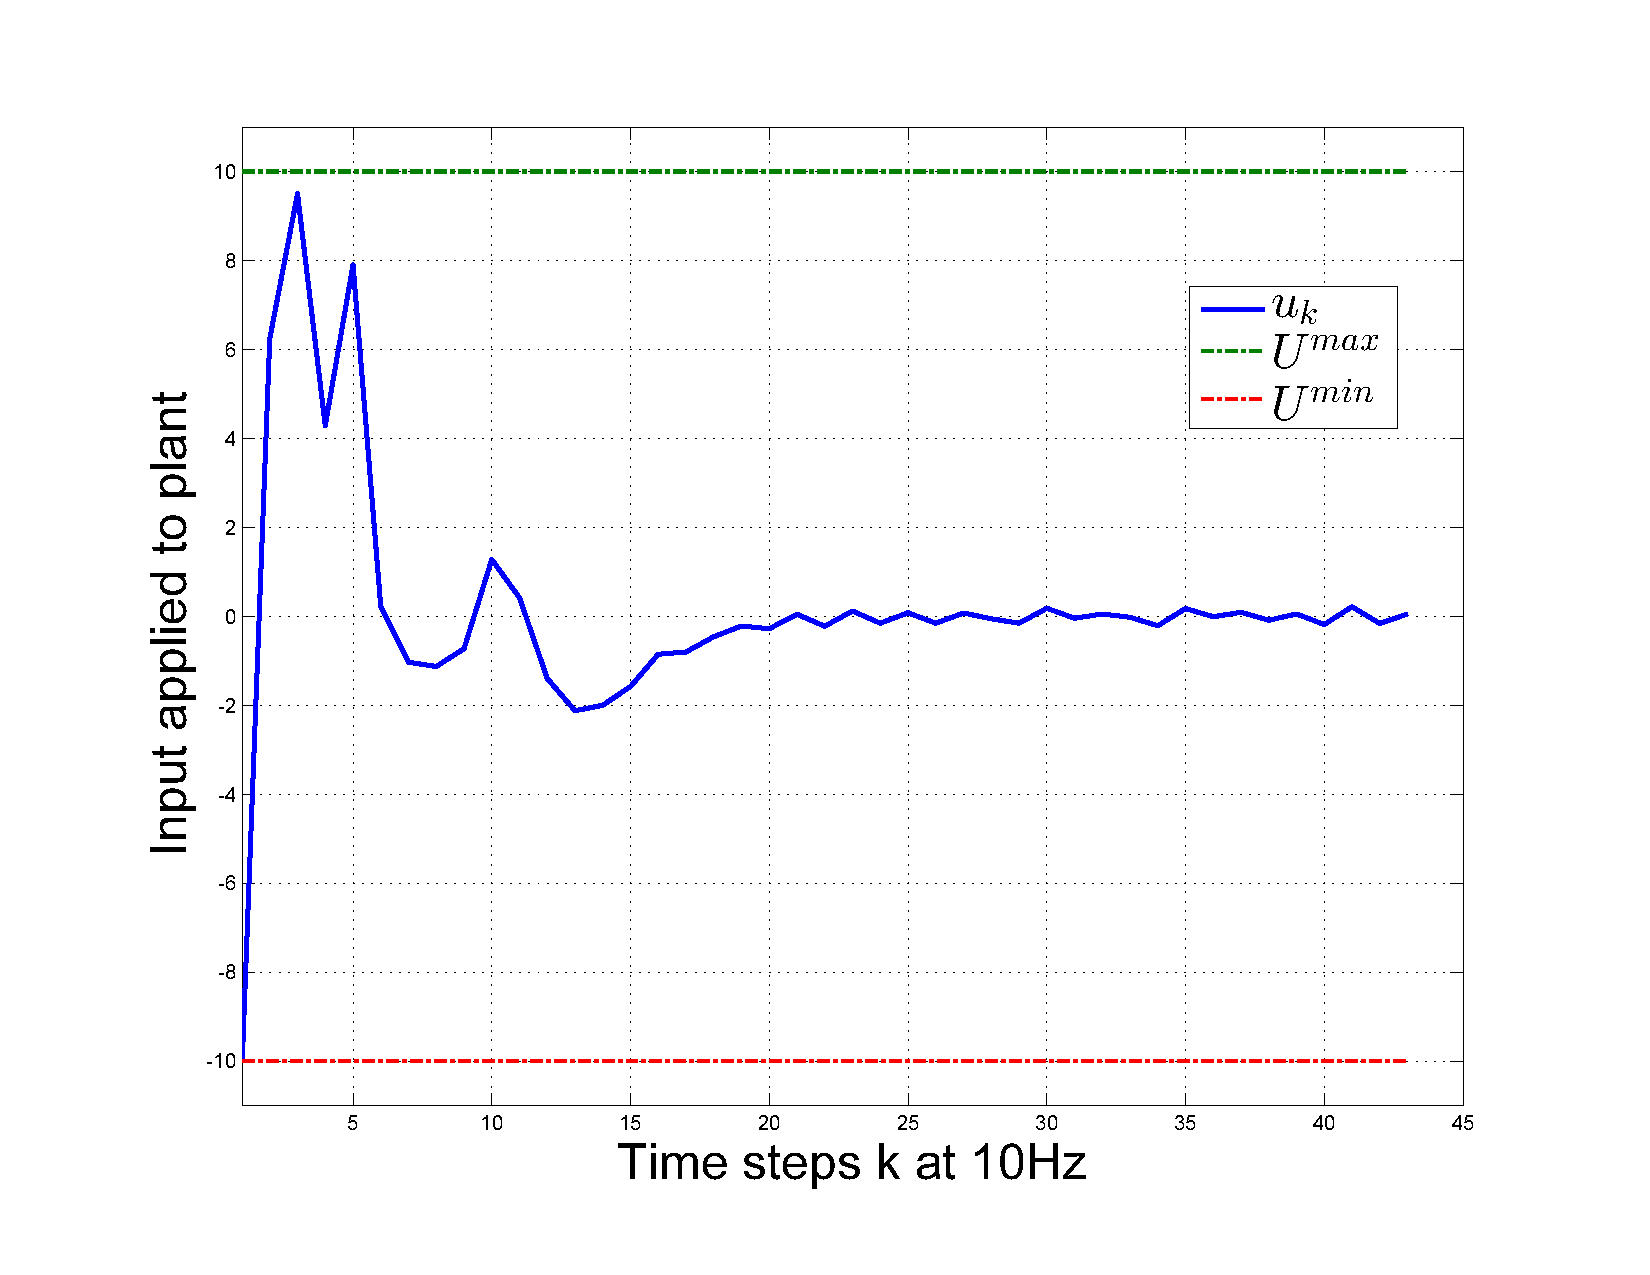
\includegraphics[width=0.49\textwidth]{figs/u_and_limits_manip.pdf}
\caption{Input to the non-linear system and its upper and lower limits.}
\label{fig:u_and_limits}
\end{figure}


